\section{Quantum Communication System}
    \begin{figure}[t]
        \begin{center}
            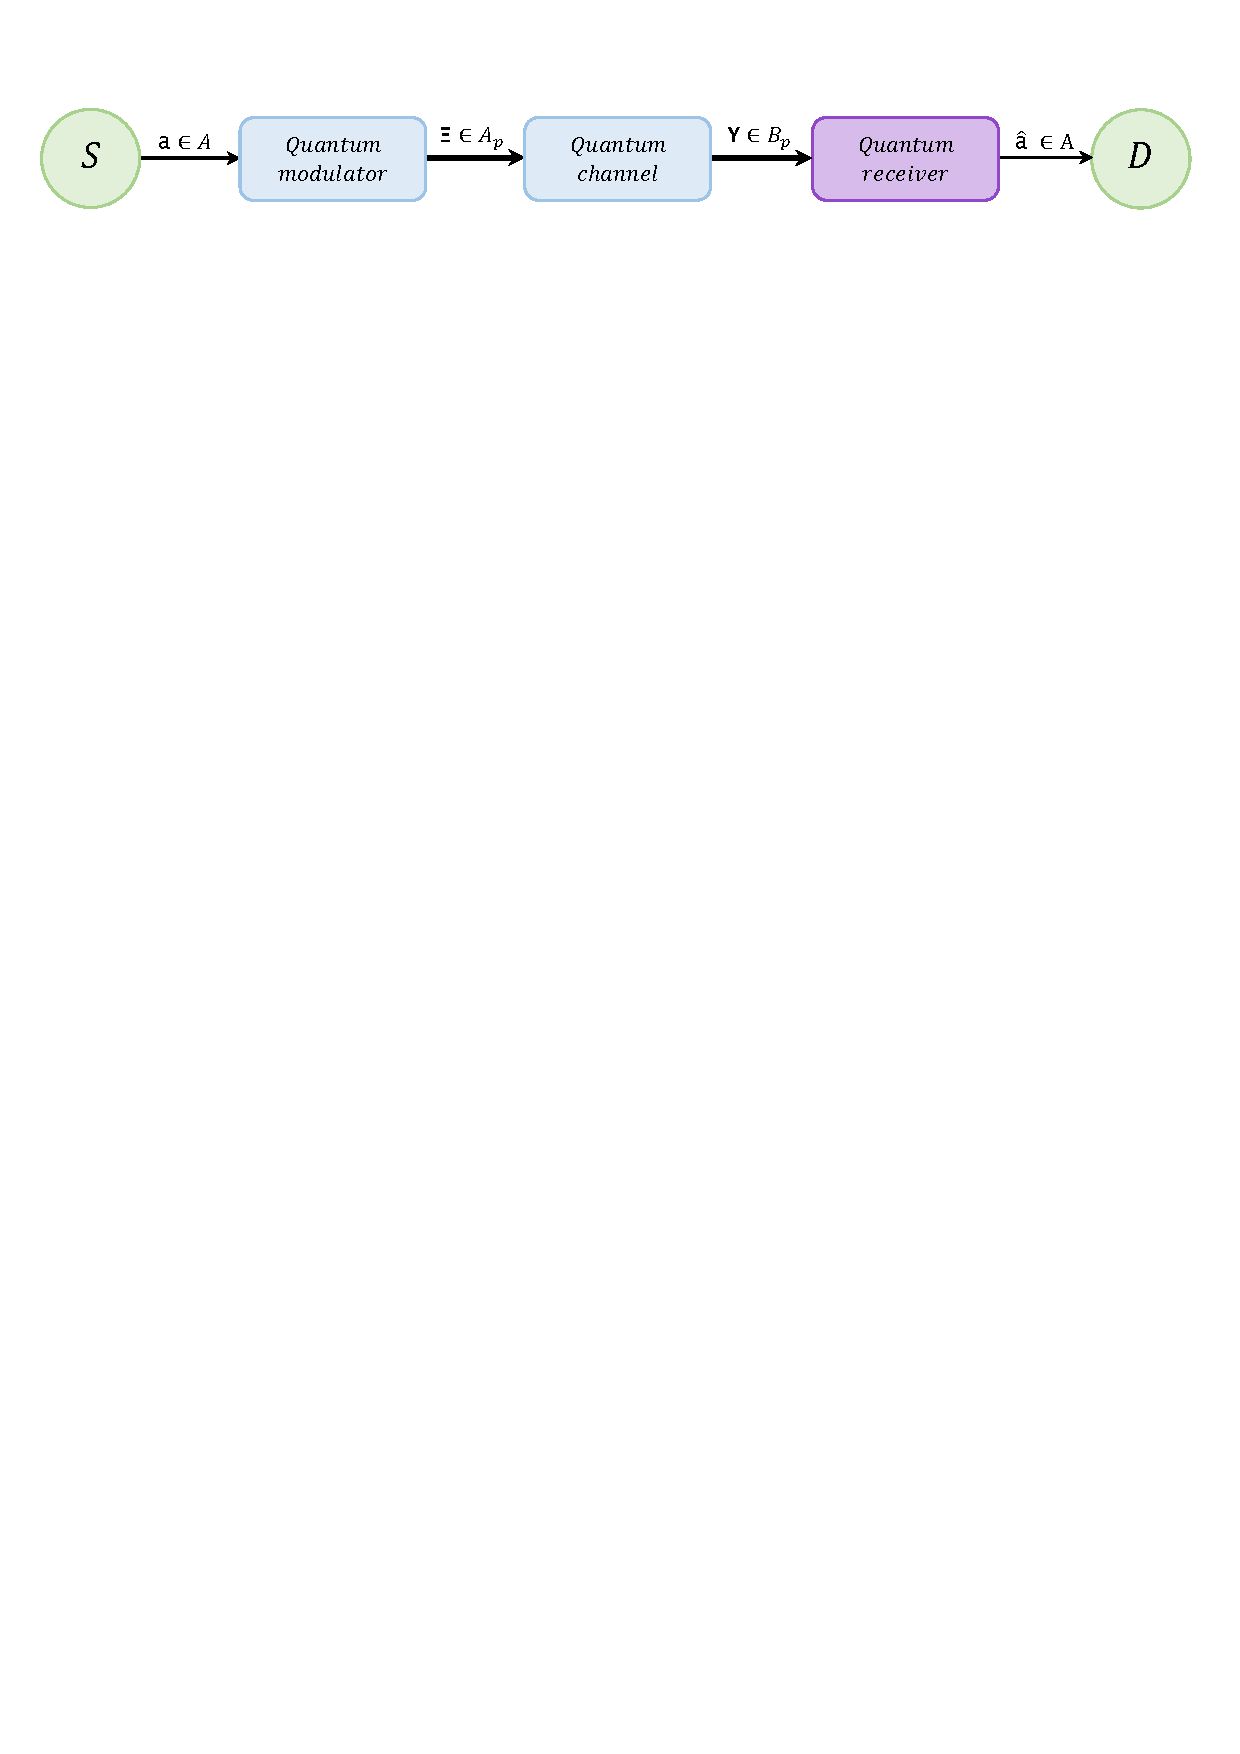
\includegraphics[width=1\textwidth]{fig3.0.pdf}
            \caption{Block-chain of a quantum communication system}
            \label{fig:3.0}
        \end{center}
    \end{figure}
    A quantum communication system can be described similarly to a classical one, as we can 
    see in figure \ref{fig:3.0}. An information source emits a unknown classical symbol 
    $\msf{a} \in \mathcal{A}$ which have to be 
    modulated with a quantum modulator that emits on the communication channel a corresponding quantum
    state $\Operator{\sXi} \in \mathcal{A}_p$. The channel can distort
    the state and deliver the state $\Operator{\sUpsilon} \in \mathcal{B}_p$ that is in general 
    different from $\Operator{\sXi}$.
    The receiver have to recognize the unknown transmitted $\msf{\hat{a}}$ as well as possible, i.e. with 
    the minimum possible error probability.
